\documentclass[a4paper]{book}
\usepackage{makeidx}
\usepackage{natbib}
\usepackage{graphicx}
\usepackage{multicol}
\usepackage{float}
\usepackage{listings}
\usepackage{color}
\usepackage{ifthen}
\usepackage[table]{xcolor}
\usepackage{textcomp}
\usepackage{alltt}
\usepackage{ifpdf}
\ifpdf
\usepackage[pdftex,
            pagebackref=true,
            colorlinks=true,
            linkcolor=blue,
            unicode
           ]{hyperref}
\else
\usepackage[ps2pdf,
            pagebackref=true,
            colorlinks=true,
            linkcolor=blue,
            unicode
           ]{hyperref}
\usepackage{pspicture}
\fi
\usepackage[utf8]{inputenc}
\usepackage{mathptmx}
\usepackage[scaled=.90]{helvet}
\usepackage{courier}
\usepackage{sectsty}
\usepackage[titles]{tocloft}
\usepackage{doxygen}
\lstset{language=C++,inputencoding=utf8,basicstyle=\footnotesize,breaklines=true,breakatwhitespace=true,tabsize=4,numbers=left }
\makeindex
\setcounter{tocdepth}{3}
\renewcommand{\footrulewidth}{0.4pt}
\renewcommand{\familydefault}{\sfdefault}
\hfuzz=15pt
\setlength{\emergencystretch}{15pt}
\hbadness=750
\tolerance=750
\begin{document}
\hypersetup{pageanchor=false,citecolor=blue}
\begin{titlepage}
\vspace*{7cm}
\begin{center}
{\Large \-Turbo\-Wavelets.\-Net }\\
\vspace*{1cm}
{\large \-Generated by Doxygen 1.7.6.1}\\
\vspace*{0.5cm}
{\small Wed Mar 15 2017 08:18:56}\\
\end{center}
\end{titlepage}
\clearemptydoublepage
\pagenumbering{roman}
\tableofcontents
\clearemptydoublepage
\pagenumbering{arabic}
\hypersetup{pageanchor=true,citecolor=blue}
\chapter{\-Turbo\-Wavelets.\-Net documentation}
\label{index}\hypertarget{index}{}\-Turbo\-Wavelets.\-Net provides very fast, flexible and compact implementations of discrete wavelet transformations in \-C\#. \-Unlike others this implementation has no limitation is sizes for the transformation (lengths like 39, 739,... are possible, not just power of two numbers) \-At the moment only floating point numbers are supported.

\-Features\-:
\begin{DoxyItemize}
\item 1\-D biorthogonal 5/3 wavelet using the lifting scheme (for arbitrary sizes, not just power of 2)
\item 2\-D biorthogonal 5/3 wavelet using the lifting scheme (for arbitrary sizes, not just power of 2)
\item 2\-D haar wavelet (for arbitrary sizes, not just power of 2)
\item 2\-D cascade sorting of coefficients (for arbitrary sizes, not just power of 2)
\item \-Scale/\-Crop coefficients in a defined grid
\item apply a deadzone
\item \-Multithreaded and threadsafe
\end{DoxyItemize}

\-Licence\-: \-M\-I\-T \-License (\-M\-I\-T) 
\chapter{\-Namespace \-Index}
\section{Packages}
Here are the packages with brief descriptions (if available)\+:\begin{DoxyCompactList}
\item\contentsline{section}{\hyperlink{namespace_turbo_wavelets}{Turbo\+Wavelets} }{\pageref{namespace_turbo_wavelets}}{}
\end{DoxyCompactList}

\chapter{\-Class \-Index}
\section{Class Hierarchy}
This inheritance list is sorted roughly, but not completely, alphabetically\+:\begin{DoxyCompactList}
\item \contentsline{section}{Turbo\+Wavelets.\+Biorthogonal53\+Wavelet1\+D\+Static}{\pageref{class_turbo_wavelets_1_1_biorthogonal53_wavelet1_d_static}}{}
\item \contentsline{section}{Turbo\+Wavelets.\+Wavelet2\+D}{\pageref{class_turbo_wavelets_1_1_wavelet2_d}}{}
\begin{DoxyCompactList}
\item \contentsline{section}{Turbo\+Wavelets.\+Biorthogonal53\+Wavelet2\+D}{\pageref{class_turbo_wavelets_1_1_biorthogonal53_wavelet2_d}}{}
\item \contentsline{section}{Turbo\+Wavelets.\+Haar\+Wavelet2\+D}{\pageref{class_turbo_wavelets_1_1_haar_wavelet2_d}}{}
\item \contentsline{section}{Turbo\+Wavelets.\+Order\+Wavelet2\+D}{\pageref{class_turbo_wavelets_1_1_order_wavelet2_d}}{}
\end{DoxyCompactList}
\end{DoxyCompactList}

\chapter{\-Class \-Index}
\section{\-Class \-List}
\-Here are the classes, structs, unions and interfaces with brief descriptions\-:\begin{DoxyCompactList}
\item\contentsline{section}{\hyperlink{class_turbo_wavelets_1_1_biorthogonal53_wavelet1_d_static}{\-Turbo\-Wavelets.\-Biorthogonal53\-Wavelet1\-D\-Static} }{\pageref{class_turbo_wavelets_1_1_biorthogonal53_wavelet1_d_static}}{}
\item\contentsline{section}{\hyperlink{class_turbo_wavelets_1_1_biorthogonal53_wavelet2_d}{\-Turbo\-Wavelets.\-Biorthogonal53\-Wavelet2\-D} }{\pageref{class_turbo_wavelets_1_1_biorthogonal53_wavelet2_d}}{}
\item\contentsline{section}{\hyperlink{class_turbo_wavelets_1_1_haar_wavelet2_d}{\-Turbo\-Wavelets.\-Haar\-Wavelet2\-D} }{\pageref{class_turbo_wavelets_1_1_haar_wavelet2_d}}{}
\item\contentsline{section}{\hyperlink{class_turbo_wavelets_1_1_order_wavelet2_d}{\-Turbo\-Wavelets.\-Order\-Wavelet2\-D} }{\pageref{class_turbo_wavelets_1_1_order_wavelet2_d}}{}
\item\contentsline{section}{\hyperlink{class_turbo_wavelets_1_1_wavelet2_d}{\-Turbo\-Wavelets.\-Wavelet2\-D} \\*\-A abstract basis class which provides common functionality for different implementations of a \char`\"{}2\-D Wavelet transformation\char`\"{} }{\pageref{class_turbo_wavelets_1_1_wavelet2_d}}{}
\end{DoxyCompactList}

\chapter{\-Namespace \-Documentation}
\hypertarget{namespace_turbo_wavelets}{\section{Package Turbo\+Wavelets}
\label{namespace_turbo_wavelets}\index{Turbo\+Wavelets@{Turbo\+Wavelets}}
}
\subsection*{Classes}
\begin{DoxyCompactItemize}
\item 
class \hyperlink{class_turbo_wavelets_1_1_biorthogonal53_wavelet1_d_static}{Biorthogonal53\+Wavelet1\+D\+Static}
\item 
class \hyperlink{class_turbo_wavelets_1_1_biorthogonal53_wavelet2_d}{Biorthogonal53\+Wavelet2\+D}
\item 
class \hyperlink{class_turbo_wavelets_1_1_haar_wavelet2_d}{Haar\+Wavelet2\+D}
\item 
class \hyperlink{class_turbo_wavelets_1_1_order_wavelet2_d}{Order\+Wavelet2\+D}
\item 
class \hyperlink{class_turbo_wavelets_1_1_wavelet2_d}{Wavelet2\+D}
\end{DoxyCompactItemize}

\chapter{\-Class \-Documentation}
\hypertarget{class_turbo_wavelets_1_1_biorthogonal53_wavelet1_d_static}{\section{\-Turbo\-Wavelets.\-Biorthogonal53\-Wavelet1\-D\-Static \-Class \-Reference}
\label{class_turbo_wavelets_1_1_biorthogonal53_wavelet1_d_static}\index{\-Turbo\-Wavelets.\-Biorthogonal53\-Wavelet1\-D\-Static@{\-Turbo\-Wavelets.\-Biorthogonal53\-Wavelet1\-D\-Static}}
}
\subsection*{\-Static \-Public \-Member \-Functions}
\begin{DoxyCompactItemize}
\item 
static void \hyperlink{class_turbo_wavelets_1_1_biorthogonal53_wavelet1_d_static_ae7119dd839f9c317e69f7cceadf6da82}{wavelet53\-\_\-1d} (float\mbox{[}$\,$\mbox{]} src, float\mbox{[}$\,$\mbox{]} dst, int length)
\begin{DoxyCompactList}\small\item\em \-A fast implementation of a 1 dimensional biorthogonal 5/3 wavelet transformation for arbitary lenghts (works for all sizes, not just power of 2) using the lifting scheme. \end{DoxyCompactList}\item 
static void \hyperlink{class_turbo_wavelets_1_1_biorthogonal53_wavelet1_d_static_a9fd288d382428a089990d1e3f6367657}{wavelet53\-\_\-1d\-\_\-inverse} (float\mbox{[}$\,$\mbox{]} src, float\mbox{[}$\,$\mbox{]} dst, int length)
\begin{DoxyCompactList}\small\item\em \-A fast implementation of a 1 dimensional biorthogonal 5/3 wavelet back-\/transformation for arbitary lenghts (works for all sizes, not just power of 2) using the lifting scheme. \end{DoxyCompactList}\end{DoxyCompactItemize}


\subsection{\-Detailed \-Description}


\-Definition at line 33 of file \-Biorthogonal53\-Wavelet1\-D\-Static.\-cs.



\subsection{\-Member \-Function \-Documentation}
\hypertarget{class_turbo_wavelets_1_1_biorthogonal53_wavelet1_d_static_ae7119dd839f9c317e69f7cceadf6da82}{\index{\-Turbo\-Wavelets\-::\-Biorthogonal53\-Wavelet1\-D\-Static@{\-Turbo\-Wavelets\-::\-Biorthogonal53\-Wavelet1\-D\-Static}!wavelet53\-\_\-1d@{wavelet53\-\_\-1d}}
\index{wavelet53\-\_\-1d@{wavelet53\-\_\-1d}!TurboWavelets::Biorthogonal53Wavelet1DStatic@{\-Turbo\-Wavelets\-::\-Biorthogonal53\-Wavelet1\-D\-Static}}
\subsubsection[{wavelet53\-\_\-1d}]{\setlength{\rightskip}{0pt plus 5cm}static void {\bf \-Turbo\-Wavelets.\-Biorthogonal53\-Wavelet1\-D\-Static.\-wavelet53\-\_\-1d} (
\begin{DoxyParamCaption}
\item[{float\mbox{[}$\,$\mbox{]}}]{src, }
\item[{float\mbox{[}$\,$\mbox{]}}]{dst, }
\item[{int}]{length}
\end{DoxyParamCaption}
)\hspace{0.3cm}{\ttfamily  \mbox{[}static\mbox{]}}}}\label{class_turbo_wavelets_1_1_biorthogonal53_wavelet1_d_static_ae7119dd839f9c317e69f7cceadf6da82}


\-A fast implementation of a 1 dimensional biorthogonal 5/3 wavelet transformation for arbitary lenghts (works for all sizes, not just power of 2) using the lifting scheme. 


\begin{DoxyParams}{\-Parameters}
{\em src} & \-The source values which should be transformed\\
\hline
{\em dst} & \-The resulting values after the transformation\\
\hline
\end{DoxyParams}
\begin{DoxyReturn}{\-Returns}
\-None
\end{DoxyReturn}


\-Definition at line 43 of file \-Biorthogonal53\-Wavelet1\-D\-Static.\-cs.

\hypertarget{class_turbo_wavelets_1_1_biorthogonal53_wavelet1_d_static_a9fd288d382428a089990d1e3f6367657}{\index{\-Turbo\-Wavelets\-::\-Biorthogonal53\-Wavelet1\-D\-Static@{\-Turbo\-Wavelets\-::\-Biorthogonal53\-Wavelet1\-D\-Static}!wavelet53\-\_\-1d\-\_\-inverse@{wavelet53\-\_\-1d\-\_\-inverse}}
\index{wavelet53\-\_\-1d\-\_\-inverse@{wavelet53\-\_\-1d\-\_\-inverse}!TurboWavelets::Biorthogonal53Wavelet1DStatic@{\-Turbo\-Wavelets\-::\-Biorthogonal53\-Wavelet1\-D\-Static}}
\subsubsection[{wavelet53\-\_\-1d\-\_\-inverse}]{\setlength{\rightskip}{0pt plus 5cm}static void {\bf \-Turbo\-Wavelets.\-Biorthogonal53\-Wavelet1\-D\-Static.\-wavelet53\-\_\-1d\-\_\-inverse} (
\begin{DoxyParamCaption}
\item[{float\mbox{[}$\,$\mbox{]}}]{src, }
\item[{float\mbox{[}$\,$\mbox{]}}]{dst, }
\item[{int}]{length}
\end{DoxyParamCaption}
)\hspace{0.3cm}{\ttfamily  \mbox{[}static\mbox{]}}}}\label{class_turbo_wavelets_1_1_biorthogonal53_wavelet1_d_static_a9fd288d382428a089990d1e3f6367657}


\-A fast implementation of a 1 dimensional biorthogonal 5/3 wavelet back-\/transformation for arbitary lenghts (works for all sizes, not just power of 2) using the lifting scheme. 


\begin{DoxyParams}{\-Parameters}
{\em src} & \-The source values which should be back-\/transformed\\
\hline
{\em dst} & \-The resulting values after the back-\/transformation\\
\hline
\end{DoxyParams}
\begin{DoxyReturn}{\-Returns}
\-None
\end{DoxyReturn}


\-Definition at line 102 of file \-Biorthogonal53\-Wavelet1\-D\-Static.\-cs.



\-The documentation for this class was generated from the following file\-:\begin{DoxyCompactItemize}
\item 
\-Turbo\-Wavelets/\hyperlink{_biorthogonal53_wavelet1_d_static_8cs}{\-Biorthogonal53\-Wavelet1\-D\-Static.\-cs}\end{DoxyCompactItemize}

\hypertarget{class_turbo_wavelets_1_1_biorthogonal53_wavelet2_d}{\section{\-Turbo\-Wavelets.\-Biorthogonal53\-Wavelet2\-D \-Class \-Reference}
\label{class_turbo_wavelets_1_1_biorthogonal53_wavelet2_d}\index{\-Turbo\-Wavelets.\-Biorthogonal53\-Wavelet2\-D@{\-Turbo\-Wavelets.\-Biorthogonal53\-Wavelet2\-D}}
}


\-Implements the two dimensional biorthogonal 5/3 wavelet transformation for arbitrary sizes.  




\-Inheritance diagram for \-Turbo\-Wavelets.\-Biorthogonal53\-Wavelet2\-D\-:
\nopagebreak
\begin{figure}[H]
\begin{center}
\leavevmode
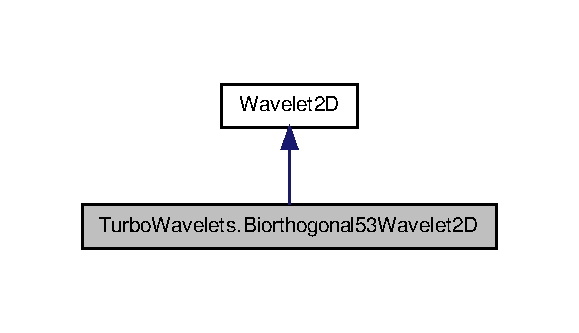
\includegraphics[width=278pt]{class_turbo_wavelets_1_1_biorthogonal53_wavelet2_d__inherit__graph}
\end{center}
\end{figure}
\subsection*{\-Public \-Member \-Functions}
\begin{DoxyCompactItemize}
\item 
\hyperlink{class_turbo_wavelets_1_1_biorthogonal53_wavelet2_d_a8783eb5b8e032cd8cf75c5a1bb80bba0}{\-Biorthogonal53\-Wavelet2\-D} (int \hyperlink{class_turbo_wavelets_1_1_wavelet2_d_aaa4b3711957fe1798980e6891331a08d}{width}, int \hyperlink{class_turbo_wavelets_1_1_wavelet2_d_afb2aa87b89b82f329357cbdc0cde18a8}{height})
\begin{DoxyCompactList}\small\item\em \-A fast implementation of a two-\/dimensional biorthogonal 5/3 wavelet transformation for arbitary lenghts (works for all sizes, not just power of 2) using the lifting scheme. \-The implementation takes advantage of multiple \-C\-P\-U cores. \end{DoxyCompactList}\item 
\hyperlink{class_turbo_wavelets_1_1_biorthogonal53_wavelet2_d_a2d9bf97c2211d5859b3a53835bea7888}{\-Biorthogonal53\-Wavelet2\-D} (int \hyperlink{class_turbo_wavelets_1_1_wavelet2_d_aaa4b3711957fe1798980e6891331a08d}{width}, int \hyperlink{class_turbo_wavelets_1_1_wavelet2_d_afb2aa87b89b82f329357cbdc0cde18a8}{height}, int \hyperlink{class_turbo_wavelets_1_1_wavelet2_d_af5148ef1a46dd5694ccea13aa8f1b9e2}{min\-Size})
\begin{DoxyCompactList}\small\item\em \-Initalizes a two dimensional wavelet transformation. \end{DoxyCompactList}\end{DoxyCompactItemize}
\subsection*{\-Protected \-Member \-Functions}
\begin{DoxyCompactItemize}
\item 
override void \hyperlink{class_turbo_wavelets_1_1_biorthogonal53_wavelet2_d_acec9bb2730e6dee78c8f6d5c8d79a523}{\-Transform\-Row} (float\mbox{[},\mbox{]} src, float\mbox{[},\mbox{]} dst, int y, int length)
\begin{DoxyCompactList}\small\item\em \-Performs a single horizontal transformation (transformation of a single row) \end{DoxyCompactList}\item 
override void \hyperlink{class_turbo_wavelets_1_1_biorthogonal53_wavelet2_d_aa93cd7f9ac110e04678a5313336fb73f}{\-Transform\-Col} (float\mbox{[},\mbox{]} src, float\mbox{[},\mbox{]} dst, int x, int length)
\begin{DoxyCompactList}\small\item\em \-Performs a single vertical transformation (transformation of a single column) \end{DoxyCompactList}\item 
override void \hyperlink{class_turbo_wavelets_1_1_biorthogonal53_wavelet2_d_a74b2789642a900fcfab4f47e023329ed}{\-Inv\-Transform\-Row} (float\mbox{[},\mbox{]} src, float\mbox{[},\mbox{]} dst, int y, int length)
\begin{DoxyCompactList}\small\item\em \-Performs a single inverse horizontal transformation (transformation of a single row) \end{DoxyCompactList}\item 
override void \hyperlink{class_turbo_wavelets_1_1_biorthogonal53_wavelet2_d_a2f52053d7f8f2da84b0ca6964481bd06}{\-Inv\-Transform\-Col} (float\mbox{[},\mbox{]} src, float\mbox{[},\mbox{]} dst, int x, int length)
\begin{DoxyCompactList}\small\item\em \-Performs a single inverse vertical transformation (transformation of a single column) \end{DoxyCompactList}\end{DoxyCompactItemize}
\subsection*{\-Protected \-Attributes}
\begin{DoxyCompactItemize}
\item 
\hypertarget{class_turbo_wavelets_1_1_biorthogonal53_wavelet2_d_a73738d4d11ccf4963deca1270953f4a0}{const int \hyperlink{class_turbo_wavelets_1_1_biorthogonal53_wavelet2_d_a73738d4d11ccf4963deca1270953f4a0}{\-Allowed\-Min\-Size} = 3}\label{class_turbo_wavelets_1_1_biorthogonal53_wavelet2_d_a73738d4d11ccf4963deca1270953f4a0}

\begin{DoxyCompactList}\small\item\em \-The allowed minimum transformation (limitation of the algorithmn implementation) $<$/supmmary$>$ \end{DoxyCompactList}\item 
const float \hyperlink{class_turbo_wavelets_1_1_biorthogonal53_wavelet2_d_a18ab552c3e524a02a6115ac6ba9dc9dd}{\-Scale} = 2.\-0f
\begin{DoxyCompactList}\small\item\em scale factor \end{DoxyCompactList}\item 
const float \hyperlink{class_turbo_wavelets_1_1_biorthogonal53_wavelet2_d_a02e708dc75d423093b1a022cc93f0388}{\-Inv\-Scale} = 0.\-5f
\begin{DoxyCompactList}\small\item\em inverse scale factor \end{DoxyCompactList}\item 
const float \hyperlink{class_turbo_wavelets_1_1_biorthogonal53_wavelet2_d_adc5fbcbea59e2154e77c9507cea584e2}{\-Mean} = 0.\-5f
\begin{DoxyCompactList}\small\item\em factor for the mean of two values \end{DoxyCompactList}\item 
const float \hyperlink{class_turbo_wavelets_1_1_biorthogonal53_wavelet2_d_a60d0110965f0ac833e932ad39b3d6f46}{\-Inv\-Mean} = 2.\-0f
\begin{DoxyCompactList}\small\item\em inverse factor for the mean of two values \end{DoxyCompactList}\item 
const float \hyperlink{class_turbo_wavelets_1_1_biorthogonal53_wavelet2_d_af84189cc1bd640074755c2ce84041c93}{\-Smooth} = 0.\-25f
\begin{DoxyCompactList}\small\item\em fraction of high-\/pass added to low-\/pass (smoothing) \end{DoxyCompactList}\item 
const float \hyperlink{class_turbo_wavelets_1_1_biorthogonal53_wavelet2_d_aef40af813a0abea998b61fdb7ce34f5d}{\-Inv\-Smooth} = 4.\-0f
\begin{DoxyCompactList}\small\item\em inverse fraction of high-\/pass added to low-\/pass (smoothing) \end{DoxyCompactList}\end{DoxyCompactItemize}


\subsection{\-Detailed \-Description}
\-Implements the two dimensional biorthogonal 5/3 wavelet transformation for arbitrary sizes. 



\-Definition at line 34 of file \-Biorthogonal53\-Wavelet2\-D.\-cs.



\subsection{\-Constructor \& \-Destructor \-Documentation}
\hypertarget{class_turbo_wavelets_1_1_biorthogonal53_wavelet2_d_a8783eb5b8e032cd8cf75c5a1bb80bba0}{\index{\-Turbo\-Wavelets\-::\-Biorthogonal53\-Wavelet2\-D@{\-Turbo\-Wavelets\-::\-Biorthogonal53\-Wavelet2\-D}!\-Biorthogonal53\-Wavelet2\-D@{\-Biorthogonal53\-Wavelet2\-D}}
\index{\-Biorthogonal53\-Wavelet2\-D@{\-Biorthogonal53\-Wavelet2\-D}!TurboWavelets::Biorthogonal53Wavelet2D@{\-Turbo\-Wavelets\-::\-Biorthogonal53\-Wavelet2\-D}}
\subsubsection[{\-Biorthogonal53\-Wavelet2\-D}]{\setlength{\rightskip}{0pt plus 5cm}{\bf \-Turbo\-Wavelets.\-Biorthogonal53\-Wavelet2\-D.\-Biorthogonal53\-Wavelet2\-D} (
\begin{DoxyParamCaption}
\item[{int}]{width, }
\item[{int}]{height}
\end{DoxyParamCaption}
)}}\label{class_turbo_wavelets_1_1_biorthogonal53_wavelet2_d_a8783eb5b8e032cd8cf75c5a1bb80bba0}


\-A fast implementation of a two-\/dimensional biorthogonal 5/3 wavelet transformation for arbitary lenghts (works for all sizes, not just power of 2) using the lifting scheme. \-The implementation takes advantage of multiple \-C\-P\-U cores. 


\begin{DoxyParams}{\-Parameters}
{\em width} & \-The width of the transformation\\
\hline
{\em height} & \-The width of the transformation\\
\hline
\end{DoxyParams}


\-Definition at line 72 of file \-Biorthogonal53\-Wavelet2\-D.\-cs.

\hypertarget{class_turbo_wavelets_1_1_biorthogonal53_wavelet2_d_a2d9bf97c2211d5859b3a53835bea7888}{\index{\-Turbo\-Wavelets\-::\-Biorthogonal53\-Wavelet2\-D@{\-Turbo\-Wavelets\-::\-Biorthogonal53\-Wavelet2\-D}!\-Biorthogonal53\-Wavelet2\-D@{\-Biorthogonal53\-Wavelet2\-D}}
\index{\-Biorthogonal53\-Wavelet2\-D@{\-Biorthogonal53\-Wavelet2\-D}!TurboWavelets::Biorthogonal53Wavelet2D@{\-Turbo\-Wavelets\-::\-Biorthogonal53\-Wavelet2\-D}}
\subsubsection[{\-Biorthogonal53\-Wavelet2\-D}]{\setlength{\rightskip}{0pt plus 5cm}{\bf \-Turbo\-Wavelets.\-Biorthogonal53\-Wavelet2\-D.\-Biorthogonal53\-Wavelet2\-D} (
\begin{DoxyParamCaption}
\item[{int}]{width, }
\item[{int}]{height, }
\item[{int}]{min\-Size}
\end{DoxyParamCaption}
)}}\label{class_turbo_wavelets_1_1_biorthogonal53_wavelet2_d_a2d9bf97c2211d5859b3a53835bea7888}


\-Initalizes a two dimensional wavelet transformation. 


\begin{DoxyParams}{\-Parameters}
{\em width} & \-The width of the transformation\\
\hline
{\em height} & \-The width of the transformation\\
\hline
{\em min\-Size} & \-Minimum width/height up to the transformation should be applied\\
\hline
\end{DoxyParams}


\-Definition at line 83 of file \-Biorthogonal53\-Wavelet2\-D.\-cs.



\subsection{\-Member \-Function \-Documentation}
\hypertarget{class_turbo_wavelets_1_1_biorthogonal53_wavelet2_d_a2f52053d7f8f2da84b0ca6964481bd06}{\index{\-Turbo\-Wavelets\-::\-Biorthogonal53\-Wavelet2\-D@{\-Turbo\-Wavelets\-::\-Biorthogonal53\-Wavelet2\-D}!\-Inv\-Transform\-Col@{\-Inv\-Transform\-Col}}
\index{\-Inv\-Transform\-Col@{\-Inv\-Transform\-Col}!TurboWavelets::Biorthogonal53Wavelet2D@{\-Turbo\-Wavelets\-::\-Biorthogonal53\-Wavelet2\-D}}
\subsubsection[{\-Inv\-Transform\-Col}]{\setlength{\rightskip}{0pt plus 5cm}override void {\bf \-Turbo\-Wavelets.\-Biorthogonal53\-Wavelet2\-D.\-Inv\-Transform\-Col} (
\begin{DoxyParamCaption}
\item[{float}]{src\mbox{[},\mbox{]}, }
\item[{float}]{dst\mbox{[},\mbox{]}, }
\item[{int}]{x, }
\item[{int}]{length}
\end{DoxyParamCaption}
)\hspace{0.3cm}{\ttfamily  \mbox{[}protected, virtual\mbox{]}}}}\label{class_turbo_wavelets_1_1_biorthogonal53_wavelet2_d_a2f52053d7f8f2da84b0ca6964481bd06}


\-Performs a single inverse vertical transformation (transformation of a single column) 


\begin{DoxyParams}{\-Parameters}
{\em src} & 2d float array on which should be used as source for the transformation\\
\hline
{\em dst} & 2d float array on which should be used as destination for the transformation\\
\hline
{\em x} & index of the row which should be transformed\\
\hline
{\em length} & number of entries to transform\\
\hline
\end{DoxyParams}


\-Reimplemented from \hyperlink{class_turbo_wavelets_1_1_wavelet2_d_a9897e5e3f830ab7ea106e6bcf367fa07}{\-Turbo\-Wavelets.\-Wavelet2\-D}.



\-Definition at line 252 of file \-Biorthogonal53\-Wavelet2\-D.\-cs.

\hypertarget{class_turbo_wavelets_1_1_biorthogonal53_wavelet2_d_a74b2789642a900fcfab4f47e023329ed}{\index{\-Turbo\-Wavelets\-::\-Biorthogonal53\-Wavelet2\-D@{\-Turbo\-Wavelets\-::\-Biorthogonal53\-Wavelet2\-D}!\-Inv\-Transform\-Row@{\-Inv\-Transform\-Row}}
\index{\-Inv\-Transform\-Row@{\-Inv\-Transform\-Row}!TurboWavelets::Biorthogonal53Wavelet2D@{\-Turbo\-Wavelets\-::\-Biorthogonal53\-Wavelet2\-D}}
\subsubsection[{\-Inv\-Transform\-Row}]{\setlength{\rightskip}{0pt plus 5cm}override void {\bf \-Turbo\-Wavelets.\-Biorthogonal53\-Wavelet2\-D.\-Inv\-Transform\-Row} (
\begin{DoxyParamCaption}
\item[{float}]{src\mbox{[},\mbox{]}, }
\item[{float}]{dst\mbox{[},\mbox{]}, }
\item[{int}]{y, }
\item[{int}]{length}
\end{DoxyParamCaption}
)\hspace{0.3cm}{\ttfamily  \mbox{[}protected, virtual\mbox{]}}}}\label{class_turbo_wavelets_1_1_biorthogonal53_wavelet2_d_a74b2789642a900fcfab4f47e023329ed}


\-Performs a single inverse horizontal transformation (transformation of a single row) 


\begin{DoxyParams}{\-Parameters}
{\em src} & 2d float array on which should be used as source for the transformation\\
\hline
{\em dst} & 2d float array on which should be used as destination for the transformation\\
\hline
{\em y} & index of the row which should be transformed\\
\hline
{\em length} & number of entries to transform\\
\hline
\end{DoxyParams}


\-Reimplemented from \hyperlink{class_turbo_wavelets_1_1_wavelet2_d_ac0b65a648f05436b54aa4d925812e1d5}{\-Turbo\-Wavelets.\-Wavelet2\-D}.



\-Definition at line 192 of file \-Biorthogonal53\-Wavelet2\-D.\-cs.

\hypertarget{class_turbo_wavelets_1_1_biorthogonal53_wavelet2_d_aa93cd7f9ac110e04678a5313336fb73f}{\index{\-Turbo\-Wavelets\-::\-Biorthogonal53\-Wavelet2\-D@{\-Turbo\-Wavelets\-::\-Biorthogonal53\-Wavelet2\-D}!\-Transform\-Col@{\-Transform\-Col}}
\index{\-Transform\-Col@{\-Transform\-Col}!TurboWavelets::Biorthogonal53Wavelet2D@{\-Turbo\-Wavelets\-::\-Biorthogonal53\-Wavelet2\-D}}
\subsubsection[{\-Transform\-Col}]{\setlength{\rightskip}{0pt plus 5cm}override void {\bf \-Turbo\-Wavelets.\-Biorthogonal53\-Wavelet2\-D.\-Transform\-Col} (
\begin{DoxyParamCaption}
\item[{float}]{src\mbox{[},\mbox{]}, }
\item[{float}]{dst\mbox{[},\mbox{]}, }
\item[{int}]{x, }
\item[{int}]{length}
\end{DoxyParamCaption}
)\hspace{0.3cm}{\ttfamily  \mbox{[}protected, virtual\mbox{]}}}}\label{class_turbo_wavelets_1_1_biorthogonal53_wavelet2_d_aa93cd7f9ac110e04678a5313336fb73f}


\-Performs a single vertical transformation (transformation of a single column) 


\begin{DoxyParams}{\-Parameters}
{\em src} & 2d float array on which should be used as source for the transformation\\
\hline
{\em dst} & 2d float array on which should be used as destination for the transformation\\
\hline
{\em x} & index of the row which should be transformed\\
\hline
{\em length} & number of entries to transform\\
\hline
\end{DoxyParams}


\-Reimplemented from \hyperlink{class_turbo_wavelets_1_1_wavelet2_d_a6a6c334fb499d248b72215001ff5e9d4}{\-Turbo\-Wavelets.\-Wavelet2\-D}.



\-Definition at line 141 of file \-Biorthogonal53\-Wavelet2\-D.\-cs.

\hypertarget{class_turbo_wavelets_1_1_biorthogonal53_wavelet2_d_acec9bb2730e6dee78c8f6d5c8d79a523}{\index{\-Turbo\-Wavelets\-::\-Biorthogonal53\-Wavelet2\-D@{\-Turbo\-Wavelets\-::\-Biorthogonal53\-Wavelet2\-D}!\-Transform\-Row@{\-Transform\-Row}}
\index{\-Transform\-Row@{\-Transform\-Row}!TurboWavelets::Biorthogonal53Wavelet2D@{\-Turbo\-Wavelets\-::\-Biorthogonal53\-Wavelet2\-D}}
\subsubsection[{\-Transform\-Row}]{\setlength{\rightskip}{0pt plus 5cm}override void {\bf \-Turbo\-Wavelets.\-Biorthogonal53\-Wavelet2\-D.\-Transform\-Row} (
\begin{DoxyParamCaption}
\item[{float}]{src\mbox{[},\mbox{]}, }
\item[{float}]{dst\mbox{[},\mbox{]}, }
\item[{int}]{y, }
\item[{int}]{length}
\end{DoxyParamCaption}
)\hspace{0.3cm}{\ttfamily  \mbox{[}protected, virtual\mbox{]}}}}\label{class_turbo_wavelets_1_1_biorthogonal53_wavelet2_d_acec9bb2730e6dee78c8f6d5c8d79a523}


\-Performs a single horizontal transformation (transformation of a single row) 


\begin{DoxyParams}{\-Parameters}
{\em src} & 2d float array on which should be used as source for the transformation\\
\hline
{\em dst} & 2d float array on which should be used as destination for the transformation\\
\hline
{\em y} & index of the row which should be transformed\\
\hline
{\em length} & number of entries to transform\\
\hline
\end{DoxyParams}


\-Reimplemented from \hyperlink{class_turbo_wavelets_1_1_wavelet2_d_af0339475762d327f9d8ec019079cdc28}{\-Turbo\-Wavelets.\-Wavelet2\-D}.



\-Definition at line 89 of file \-Biorthogonal53\-Wavelet2\-D.\-cs.



\subsection{\-Member \-Data \-Documentation}
\hypertarget{class_turbo_wavelets_1_1_biorthogonal53_wavelet2_d_a60d0110965f0ac833e932ad39b3d6f46}{\index{\-Turbo\-Wavelets\-::\-Biorthogonal53\-Wavelet2\-D@{\-Turbo\-Wavelets\-::\-Biorthogonal53\-Wavelet2\-D}!\-Inv\-Mean@{\-Inv\-Mean}}
\index{\-Inv\-Mean@{\-Inv\-Mean}!TurboWavelets::Biorthogonal53Wavelet2D@{\-Turbo\-Wavelets\-::\-Biorthogonal53\-Wavelet2\-D}}
\subsubsection[{\-Inv\-Mean}]{\setlength{\rightskip}{0pt plus 5cm}const float {\bf \-Turbo\-Wavelets.\-Biorthogonal53\-Wavelet2\-D.\-Inv\-Mean} = 2.\-0f\hspace{0.3cm}{\ttfamily  \mbox{[}protected\mbox{]}}}}\label{class_turbo_wavelets_1_1_biorthogonal53_wavelet2_d_a60d0110965f0ac833e932ad39b3d6f46}


inverse factor for the mean of two values 



\-Definition at line 55 of file \-Biorthogonal53\-Wavelet2\-D.\-cs.

\hypertarget{class_turbo_wavelets_1_1_biorthogonal53_wavelet2_d_a02e708dc75d423093b1a022cc93f0388}{\index{\-Turbo\-Wavelets\-::\-Biorthogonal53\-Wavelet2\-D@{\-Turbo\-Wavelets\-::\-Biorthogonal53\-Wavelet2\-D}!\-Inv\-Scale@{\-Inv\-Scale}}
\index{\-Inv\-Scale@{\-Inv\-Scale}!TurboWavelets::Biorthogonal53Wavelet2D@{\-Turbo\-Wavelets\-::\-Biorthogonal53\-Wavelet2\-D}}
\subsubsection[{\-Inv\-Scale}]{\setlength{\rightskip}{0pt plus 5cm}const float {\bf \-Turbo\-Wavelets.\-Biorthogonal53\-Wavelet2\-D.\-Inv\-Scale} = 0.\-5f\hspace{0.3cm}{\ttfamily  \mbox{[}protected\mbox{]}}}}\label{class_turbo_wavelets_1_1_biorthogonal53_wavelet2_d_a02e708dc75d423093b1a022cc93f0388}


inverse scale factor 



\-Definition at line 47 of file \-Biorthogonal53\-Wavelet2\-D.\-cs.

\hypertarget{class_turbo_wavelets_1_1_biorthogonal53_wavelet2_d_aef40af813a0abea998b61fdb7ce34f5d}{\index{\-Turbo\-Wavelets\-::\-Biorthogonal53\-Wavelet2\-D@{\-Turbo\-Wavelets\-::\-Biorthogonal53\-Wavelet2\-D}!\-Inv\-Smooth@{\-Inv\-Smooth}}
\index{\-Inv\-Smooth@{\-Inv\-Smooth}!TurboWavelets::Biorthogonal53Wavelet2D@{\-Turbo\-Wavelets\-::\-Biorthogonal53\-Wavelet2\-D}}
\subsubsection[{\-Inv\-Smooth}]{\setlength{\rightskip}{0pt plus 5cm}const float {\bf \-Turbo\-Wavelets.\-Biorthogonal53\-Wavelet2\-D.\-Inv\-Smooth} = 4.\-0f\hspace{0.3cm}{\ttfamily  \mbox{[}protected\mbox{]}}}}\label{class_turbo_wavelets_1_1_biorthogonal53_wavelet2_d_aef40af813a0abea998b61fdb7ce34f5d}


inverse fraction of high-\/pass added to low-\/pass (smoothing) 



\-Definition at line 63 of file \-Biorthogonal53\-Wavelet2\-D.\-cs.

\hypertarget{class_turbo_wavelets_1_1_biorthogonal53_wavelet2_d_adc5fbcbea59e2154e77c9507cea584e2}{\index{\-Turbo\-Wavelets\-::\-Biorthogonal53\-Wavelet2\-D@{\-Turbo\-Wavelets\-::\-Biorthogonal53\-Wavelet2\-D}!\-Mean@{\-Mean}}
\index{\-Mean@{\-Mean}!TurboWavelets::Biorthogonal53Wavelet2D@{\-Turbo\-Wavelets\-::\-Biorthogonal53\-Wavelet2\-D}}
\subsubsection[{\-Mean}]{\setlength{\rightskip}{0pt plus 5cm}const float {\bf \-Turbo\-Wavelets.\-Biorthogonal53\-Wavelet2\-D.\-Mean} = 0.\-5f\hspace{0.3cm}{\ttfamily  \mbox{[}protected\mbox{]}}}}\label{class_turbo_wavelets_1_1_biorthogonal53_wavelet2_d_adc5fbcbea59e2154e77c9507cea584e2}


factor for the mean of two values 



\-Definition at line 51 of file \-Biorthogonal53\-Wavelet2\-D.\-cs.

\hypertarget{class_turbo_wavelets_1_1_biorthogonal53_wavelet2_d_a18ab552c3e524a02a6115ac6ba9dc9dd}{\index{\-Turbo\-Wavelets\-::\-Biorthogonal53\-Wavelet2\-D@{\-Turbo\-Wavelets\-::\-Biorthogonal53\-Wavelet2\-D}!\-Scale@{\-Scale}}
\index{\-Scale@{\-Scale}!TurboWavelets::Biorthogonal53Wavelet2D@{\-Turbo\-Wavelets\-::\-Biorthogonal53\-Wavelet2\-D}}
\subsubsection[{\-Scale}]{\setlength{\rightskip}{0pt plus 5cm}const float {\bf \-Turbo\-Wavelets.\-Biorthogonal53\-Wavelet2\-D.\-Scale} = 2.\-0f\hspace{0.3cm}{\ttfamily  \mbox{[}protected\mbox{]}}}}\label{class_turbo_wavelets_1_1_biorthogonal53_wavelet2_d_a18ab552c3e524a02a6115ac6ba9dc9dd}


scale factor 



\-Definition at line 43 of file \-Biorthogonal53\-Wavelet2\-D.\-cs.

\hypertarget{class_turbo_wavelets_1_1_biorthogonal53_wavelet2_d_af84189cc1bd640074755c2ce84041c93}{\index{\-Turbo\-Wavelets\-::\-Biorthogonal53\-Wavelet2\-D@{\-Turbo\-Wavelets\-::\-Biorthogonal53\-Wavelet2\-D}!\-Smooth@{\-Smooth}}
\index{\-Smooth@{\-Smooth}!TurboWavelets::Biorthogonal53Wavelet2D@{\-Turbo\-Wavelets\-::\-Biorthogonal53\-Wavelet2\-D}}
\subsubsection[{\-Smooth}]{\setlength{\rightskip}{0pt plus 5cm}const float {\bf \-Turbo\-Wavelets.\-Biorthogonal53\-Wavelet2\-D.\-Smooth} = 0.\-25f\hspace{0.3cm}{\ttfamily  \mbox{[}protected\mbox{]}}}}\label{class_turbo_wavelets_1_1_biorthogonal53_wavelet2_d_af84189cc1bd640074755c2ce84041c93}


fraction of high-\/pass added to low-\/pass (smoothing) 



\-Definition at line 59 of file \-Biorthogonal53\-Wavelet2\-D.\-cs.



\-The documentation for this class was generated from the following file\-:\begin{DoxyCompactItemize}
\item 
\-Turbo\-Wavelets/\-Biorthogonal53\-Wavelet2\-D.\-cs\end{DoxyCompactItemize}

\hypertarget{class_turbo_wavelets_1_1_haar_wavelet2_d}{\section{\-Turbo\-Wavelets.\-Haar\-Wavelet2\-D \-Class \-Reference}
\label{class_turbo_wavelets_1_1_haar_wavelet2_d}\index{\-Turbo\-Wavelets.\-Haar\-Wavelet2\-D@{\-Turbo\-Wavelets.\-Haar\-Wavelet2\-D}}
}


\-Inheritance diagram for \-Turbo\-Wavelets.\-Haar\-Wavelet2\-D\-:
\nopagebreak
\begin{figure}[H]
\begin{center}
\leavevmode
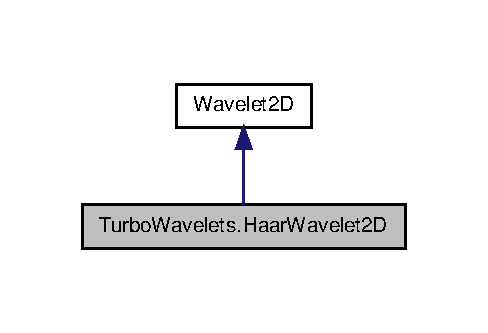
\includegraphics[width=234pt]{class_turbo_wavelets_1_1_haar_wavelet2_d__inherit__graph}
\end{center}
\end{figure}
\subsection*{\-Public \-Member \-Functions}
\begin{DoxyCompactItemize}
\item 
\hyperlink{class_turbo_wavelets_1_1_haar_wavelet2_d_ab55a20658fe1f22b6e756418b4e1dc29}{\-Haar\-Wavelet2\-D} (int width, int height)
\begin{DoxyCompactList}\small\item\em \-A fast implementation of a two-\/dimensional haar transformation for arbitary lenghts (works for all sizes, not just power of 2) \-The implementation takes advantage of multiple \-C\-P\-U cores. \end{DoxyCompactList}\item 
\hyperlink{class_turbo_wavelets_1_1_haar_wavelet2_d_a8064166eec2c0a4b66378896b882bd47}{\-Haar\-Wavelet2\-D} (int width, int height, int min\-Size)
\begin{DoxyCompactList}\small\item\em \-A fast implementation of a two-\/dimensional haar transformation for arbitary lenghts (works for all sizes, not just power of 2) \-The implementation takes advantage of multiple \-C\-P\-U cores. \end{DoxyCompactList}\end{DoxyCompactItemize}


\subsection{\-Detailed \-Description}


\-Definition at line 32 of file \-Haar\-Wavelet2\-D.\-cs.



\subsection{\-Constructor \& \-Destructor \-Documentation}
\hypertarget{class_turbo_wavelets_1_1_haar_wavelet2_d_ab55a20658fe1f22b6e756418b4e1dc29}{\index{\-Turbo\-Wavelets\-::\-Haar\-Wavelet2\-D@{\-Turbo\-Wavelets\-::\-Haar\-Wavelet2\-D}!\-Haar\-Wavelet2\-D@{\-Haar\-Wavelet2\-D}}
\index{\-Haar\-Wavelet2\-D@{\-Haar\-Wavelet2\-D}!TurboWavelets::HaarWavelet2D@{\-Turbo\-Wavelets\-::\-Haar\-Wavelet2\-D}}
\subsubsection[{\-Haar\-Wavelet2\-D}]{\setlength{\rightskip}{0pt plus 5cm}{\bf \-Turbo\-Wavelets.\-Haar\-Wavelet2\-D.\-Haar\-Wavelet2\-D} (
\begin{DoxyParamCaption}
\item[{int}]{width, }
\item[{int}]{height}
\end{DoxyParamCaption}
)}}\label{class_turbo_wavelets_1_1_haar_wavelet2_d_ab55a20658fe1f22b6e756418b4e1dc29}


\-A fast implementation of a two-\/dimensional haar transformation for arbitary lenghts (works for all sizes, not just power of 2) \-The implementation takes advantage of multiple \-C\-P\-U cores. 


\begin{DoxyParams}{\-Parameters}
{\em width} & \-The width of the transformation\\
\hline
{\em height} & \-The width of the transformation\\
\hline
\end{DoxyParams}


\-Definition at line 47 of file \-Haar\-Wavelet2\-D.\-cs.

\hypertarget{class_turbo_wavelets_1_1_haar_wavelet2_d_a8064166eec2c0a4b66378896b882bd47}{\index{\-Turbo\-Wavelets\-::\-Haar\-Wavelet2\-D@{\-Turbo\-Wavelets\-::\-Haar\-Wavelet2\-D}!\-Haar\-Wavelet2\-D@{\-Haar\-Wavelet2\-D}}
\index{\-Haar\-Wavelet2\-D@{\-Haar\-Wavelet2\-D}!TurboWavelets::HaarWavelet2D@{\-Turbo\-Wavelets\-::\-Haar\-Wavelet2\-D}}
\subsubsection[{\-Haar\-Wavelet2\-D}]{\setlength{\rightskip}{0pt plus 5cm}{\bf \-Turbo\-Wavelets.\-Haar\-Wavelet2\-D.\-Haar\-Wavelet2\-D} (
\begin{DoxyParamCaption}
\item[{int}]{width, }
\item[{int}]{height, }
\item[{int}]{min\-Size}
\end{DoxyParamCaption}
)}}\label{class_turbo_wavelets_1_1_haar_wavelet2_d_a8064166eec2c0a4b66378896b882bd47}


\-A fast implementation of a two-\/dimensional haar transformation for arbitary lenghts (works for all sizes, not just power of 2) \-The implementation takes advantage of multiple \-C\-P\-U cores. 


\begin{DoxyParams}{\-Parameters}
{\em width} & \-The width of the transformation\\
\hline
{\em height} & \-The width of the transformation\\
\hline
{\em min\-Size} & \-Minimum width/height up to the transformation should be applied\\
\hline
\end{DoxyParams}


\-Definition at line 60 of file \-Haar\-Wavelet2\-D.\-cs.



\-The documentation for this class was generated from the following file\-:\begin{DoxyCompactItemize}
\item 
\-Turbo\-Wavelets/\-Haar\-Wavelet2\-D.\-cs\end{DoxyCompactItemize}

\hypertarget{class_turbo_wavelets_1_1_order_wavelet2_d}{\section{\-Turbo\-Wavelets.\-Order\-Wavelet2\-D \-Class \-Reference}
\label{class_turbo_wavelets_1_1_order_wavelet2_d}\index{\-Turbo\-Wavelets.\-Order\-Wavelet2\-D@{\-Turbo\-Wavelets.\-Order\-Wavelet2\-D}}
}


\-Inheritance diagram for \-Turbo\-Wavelets.\-Order\-Wavelet2\-D\-:
\nopagebreak
\begin{figure}[H]
\begin{center}
\leavevmode
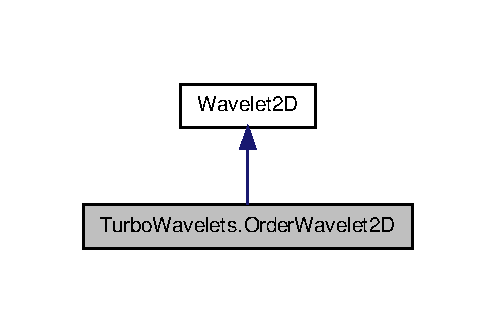
\includegraphics[width=238pt]{class_turbo_wavelets_1_1_order_wavelet2_d__inherit__graph}
\end{center}
\end{figure}


\-Collaboration diagram for \-Turbo\-Wavelets.\-Order\-Wavelet2\-D\-:
\nopagebreak
\begin{figure}[H]
\begin{center}
\leavevmode
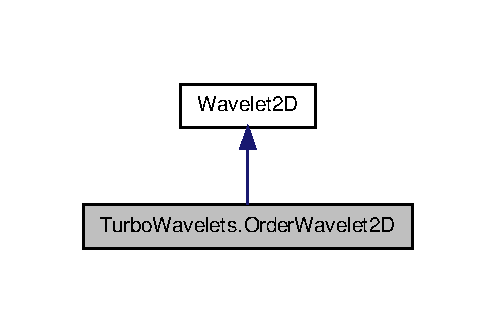
\includegraphics[width=238pt]{class_turbo_wavelets_1_1_order_wavelet2_d__coll__graph}
\end{center}
\end{figure}
\subsection*{\-Public \-Member \-Functions}
\begin{DoxyCompactItemize}
\item 
\hyperlink{class_turbo_wavelets_1_1_order_wavelet2_d_aed357d3d66affbf094ee6e104ac75f1f}{\-Order\-Wavelet2\-D} (int width, int height)
\begin{DoxyCompactList}\small\item\em \-A fast implementation of a two-\/dimensional ordering transformation for arbitary lenghts (works for all sizes, not just power of 2) \-This does not perform a complete wavelet transformation. \-It just does the cascade ordering of the values. \-The implementation takes advantage of multiple \-C\-P\-U cores. \end{DoxyCompactList}\item 
\hyperlink{class_turbo_wavelets_1_1_order_wavelet2_d_a22aec9d1c8fd7f56ac480a305ce4e9cd}{\-Order\-Wavelet2\-D} (int width, int height, int min\-Size)
\begin{DoxyCompactList}\small\item\em \-A fast implementation of a two-\/dimensional ordering transformation for arbitary lenghts (works for all sizes, not just power of 2) \-This does not perform a complete wavelet transformation. \-It just does the cascade ordering of the values. \-The implementation takes advantage of multiple \-C\-P\-U cores. \end{DoxyCompactList}\end{DoxyCompactItemize}
\subsection*{\-Protected \-Member \-Functions}
\begin{DoxyCompactItemize}
\item 
\hypertarget{class_turbo_wavelets_1_1_order_wavelet2_d_af45baa14b0d867362b989db7d41f14dc}{override void {\bfseries \-Transform\-Row} (float\mbox{[},\mbox{]} src, float\mbox{[},\mbox{]} dst, int y, int length)}\label{class_turbo_wavelets_1_1_order_wavelet2_d_af45baa14b0d867362b989db7d41f14dc}

\item 
\hypertarget{class_turbo_wavelets_1_1_order_wavelet2_d_a94c72dd8852fe900901bcffd12c37272}{override void {\bfseries \-Transform\-Col} (float\mbox{[},\mbox{]} src, float\mbox{[},\mbox{]} dst, int x, int length)}\label{class_turbo_wavelets_1_1_order_wavelet2_d_a94c72dd8852fe900901bcffd12c37272}

\item 
\hypertarget{class_turbo_wavelets_1_1_order_wavelet2_d_a67a15c5e174f2bf762d153a976f86b36}{override void {\bfseries \-Inv\-Transform\-Row} (float\mbox{[},\mbox{]} src, float\mbox{[},\mbox{]} dst, int y, int length)}\label{class_turbo_wavelets_1_1_order_wavelet2_d_a67a15c5e174f2bf762d153a976f86b36}

\item 
\hypertarget{class_turbo_wavelets_1_1_order_wavelet2_d_ae7e013e9ee79f1d0932de6fa2e1854de}{override void {\bfseries \-Inv\-Transform\-Col} (float\mbox{[},\mbox{]} src, float\mbox{[},\mbox{]} dst, int x, int length)}\label{class_turbo_wavelets_1_1_order_wavelet2_d_ae7e013e9ee79f1d0932de6fa2e1854de}

\end{DoxyCompactItemize}


\subsection{\-Detailed \-Description}


\-Definition at line 33 of file \-Order\-Wavelet2\-D.\-cs.



\subsection{\-Constructor \& \-Destructor \-Documentation}
\hypertarget{class_turbo_wavelets_1_1_order_wavelet2_d_aed357d3d66affbf094ee6e104ac75f1f}{\index{\-Turbo\-Wavelets\-::\-Order\-Wavelet2\-D@{\-Turbo\-Wavelets\-::\-Order\-Wavelet2\-D}!\-Order\-Wavelet2\-D@{\-Order\-Wavelet2\-D}}
\index{\-Order\-Wavelet2\-D@{\-Order\-Wavelet2\-D}!TurboWavelets::OrderWavelet2D@{\-Turbo\-Wavelets\-::\-Order\-Wavelet2\-D}}
\subsubsection[{\-Order\-Wavelet2\-D}]{\setlength{\rightskip}{0pt plus 5cm}{\bf \-Turbo\-Wavelets.\-Order\-Wavelet2\-D.\-Order\-Wavelet2\-D} (
\begin{DoxyParamCaption}
\item[{int}]{width, }
\item[{int}]{height}
\end{DoxyParamCaption}
)}}\label{class_turbo_wavelets_1_1_order_wavelet2_d_aed357d3d66affbf094ee6e104ac75f1f}


\-A fast implementation of a two-\/dimensional ordering transformation for arbitary lenghts (works for all sizes, not just power of 2) \-This does not perform a complete wavelet transformation. \-It just does the cascade ordering of the values. \-The implementation takes advantage of multiple \-C\-P\-U cores. 


\begin{DoxyParams}{\-Parameters}
{\em width} & \-The width of the transformation\\
\hline
{\em height} & \-The width of the transformation\\
\hline
\end{DoxyParams}


\-Definition at line 44 of file \-Order\-Wavelet2\-D.\-cs.

\hypertarget{class_turbo_wavelets_1_1_order_wavelet2_d_a22aec9d1c8fd7f56ac480a305ce4e9cd}{\index{\-Turbo\-Wavelets\-::\-Order\-Wavelet2\-D@{\-Turbo\-Wavelets\-::\-Order\-Wavelet2\-D}!\-Order\-Wavelet2\-D@{\-Order\-Wavelet2\-D}}
\index{\-Order\-Wavelet2\-D@{\-Order\-Wavelet2\-D}!TurboWavelets::OrderWavelet2D@{\-Turbo\-Wavelets\-::\-Order\-Wavelet2\-D}}
\subsubsection[{\-Order\-Wavelet2\-D}]{\setlength{\rightskip}{0pt plus 5cm}{\bf \-Turbo\-Wavelets.\-Order\-Wavelet2\-D.\-Order\-Wavelet2\-D} (
\begin{DoxyParamCaption}
\item[{int}]{width, }
\item[{int}]{height, }
\item[{int}]{min\-Size}
\end{DoxyParamCaption}
)}}\label{class_turbo_wavelets_1_1_order_wavelet2_d_a22aec9d1c8fd7f56ac480a305ce4e9cd}


\-A fast implementation of a two-\/dimensional ordering transformation for arbitary lenghts (works for all sizes, not just power of 2) \-This does not perform a complete wavelet transformation. \-It just does the cascade ordering of the values. \-The implementation takes advantage of multiple \-C\-P\-U cores. 


\begin{DoxyParams}{\-Parameters}
{\em width} & \-The width of the transformation\\
\hline
{\em height} & \-The width of the transformation\\
\hline
{\em min\-Size} & \-Minimum width/height up to the transformation should be applied\\
\hline
\end{DoxyParams}


\-Definition at line 59 of file \-Order\-Wavelet2\-D.\-cs.



\-The documentation for this class was generated from the following file\-:\begin{DoxyCompactItemize}
\item 
\-Turbo\-Wavelets/\-Order\-Wavelet2\-D.\-cs\end{DoxyCompactItemize}

\hypertarget{class_turbo_wavelets_1_1_wavelet2_d}{\section{\-Turbo\-Wavelets.\-Wavelet2\-D \-Class \-Reference}
\label{class_turbo_wavelets_1_1_wavelet2_d}\index{\-Turbo\-Wavelets.\-Wavelet2\-D@{\-Turbo\-Wavelets.\-Wavelet2\-D}}
}


\-A abstract basis class which provides common functionality for different implementations of a \char`\"{}2\-D Wavelet transformation\char`\"{}.  




\-Inheritance diagram for \-Turbo\-Wavelets.\-Wavelet2\-D\-:
\nopagebreak
\begin{figure}[H]
\begin{center}
\leavevmode
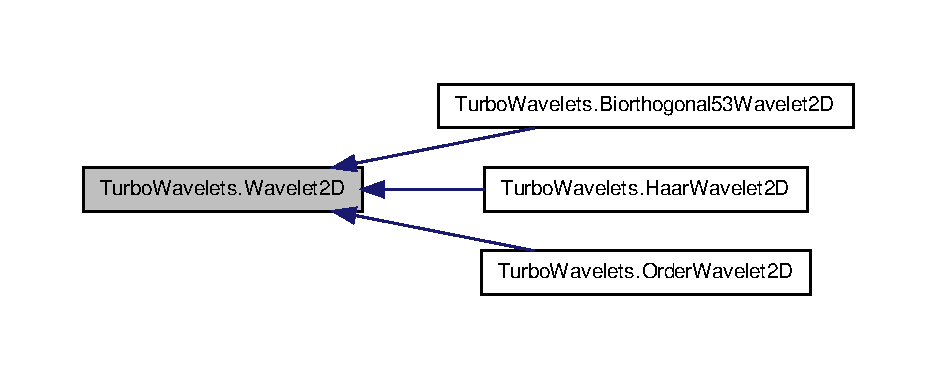
\includegraphics[width=350pt]{class_turbo_wavelets_1_1_wavelet2_d__inherit__graph}
\end{center}
\end{figure}
\subsection*{\-Public \-Member \-Functions}
\begin{DoxyCompactItemize}
\item 
\hypertarget{class_turbo_wavelets_1_1_wavelet2_d_aec52fe74aa08e073119064ef4ac3fe93}{delegate bool \hyperlink{class_turbo_wavelets_1_1_wavelet2_d_aec52fe74aa08e073119064ef4ac3fe93}{\-Progress\-Delegate} (float progress)}\label{class_turbo_wavelets_1_1_wavelet2_d_aec52fe74aa08e073119064ef4ac3fe93}

\begin{DoxyCompactList}\small\item\em \-Prototype of a delegate called to inform caller about progress and to provide possibility to abort $<$/summary. \end{DoxyCompactList}\item 
\hyperlink{class_turbo_wavelets_1_1_wavelet2_d_a5156da3a3376121d64967dd8cd75725b}{\-Wavelet2\-D} (int \hyperlink{class_turbo_wavelets_1_1_wavelet2_d_af5148ef1a46dd5694ccea13aa8f1b9e2}{min\-Size}, int \hyperlink{class_turbo_wavelets_1_1_wavelet2_d_a949bac2b4f540092cf7cc8916968cdc0}{allowed\-Min\-Size}, int \hyperlink{class_turbo_wavelets_1_1_wavelet2_d_aaa4b3711957fe1798980e6891331a08d}{width}, int \hyperlink{class_turbo_wavelets_1_1_wavelet2_d_afb2aa87b89b82f329357cbdc0cde18a8}{height})
\begin{DoxyCompactList}\small\item\em \-Initalizes a two dimensional wavelet cascade transformation. \-By the transformation the data is split up in a high-\/ and a low-\/pass. \-The low-\/pass data is repeatedly transformed again until the horizontal or vertical length reaches \char`\"{}min\-Size\char`\"{}. \end{DoxyCompactList}\item 
void \hyperlink{class_turbo_wavelets_1_1_wavelet2_d_a727e557f207cf861b10c38f1f1a91b52}{\-Flush\-Cache} ()
\begin{DoxyCompactList}\small\item\em \-Frees all cached memory. \end{DoxyCompactList}\item 
virtual void \hyperlink{class_turbo_wavelets_1_1_wavelet2_d_ac647a989c2b66ca08a8b7e4196cbc547}{\-Transform\-Isotropic2\-D} (float\mbox{[},\mbox{]} src, \hyperlink{class_turbo_wavelets_1_1_wavelet2_d_aec52fe74aa08e073119064ef4ac3fe93}{\-Progress\-Delegate} progress\-Delegate=null)
\begin{DoxyCompactList}\small\item\em \-Perfroms a two dimensional isotropic wavelet transformation for an array. \-The result is copied back to the declared array. \end{DoxyCompactList}\item 
virtual void \hyperlink{class_turbo_wavelets_1_1_wavelet2_d_ac1644fb0d5f8a2ba8f265b445cba454b}{\-Backtransform\-Isotropic2\-D} (float\mbox{[},\mbox{]} src, \hyperlink{class_turbo_wavelets_1_1_wavelet2_d_aec52fe74aa08e073119064ef4ac3fe93}{\-Progress\-Delegate} progress\-Delegate=null)
\begin{DoxyCompactList}\small\item\em \-Perfroms a two dimensional isotropic wavelet transformation for an array. \-The result is copied back to the declared array. \end{DoxyCompactList}\item 
virtual void \hyperlink{class_turbo_wavelets_1_1_wavelet2_d_a55e3f96cb79da6cc4621ccc1118a0d6f}{\-Scale\-Coefficients} (float\mbox{[},\mbox{]} src, float\mbox{[}$\,$\mbox{]} scale\-Factors, int grid\-Size, \hyperlink{class_turbo_wavelets_1_1_wavelet2_d_aec52fe74aa08e073119064ef4ac3fe93}{\-Progress\-Delegate} progress\-Delegate=null)
\begin{DoxyCompactList}\small\item\em \-Scales the n (length of the scale\-Factors array) greatest coefficinets (for a defined grid size) by the value declared in scale\-Factors. \end{DoxyCompactList}\item 
virtual void \hyperlink{class_turbo_wavelets_1_1_wavelet2_d_aa1e399d2ab5f85843185a2895bf7f7ad}{\-Crop\-Coefficients} (float\mbox{[},\mbox{]} src, int n, int grid\-Size, \hyperlink{class_turbo_wavelets_1_1_wavelet2_d_aec52fe74aa08e073119064ef4ac3fe93}{\-Progress\-Delegate} progress\-Delegate=null)
\begin{DoxyCompactList}\small\item\em \-Set all but the greatest n coefficient to zero in the defined grid size. \end{DoxyCompactList}\item 
virtual void \hyperlink{class_turbo_wavelets_1_1_wavelet2_d_a9abbbf0cffd0d8dca5d78d6ad4dad399}{\-Crop\-Coefficients} (float\mbox{[},\mbox{]} src, float min\-Absolute\-Value, \hyperlink{class_turbo_wavelets_1_1_wavelet2_d_aec52fe74aa08e073119064ef4ac3fe93}{\-Progress\-Delegate} progress\-Delegate=null)
\begin{DoxyCompactList}\small\item\em \-Set all coefficient with an absolute value smaller then \char`\"{}min\-Absolute\-Value\char`\"{} to zero (deadzone) \end{DoxyCompactList}\item 
virtual void \hyperlink{class_turbo_wavelets_1_1_wavelet2_d_ad25227565f3b5e5953e951ad5b375654}{get\-Coefficients\-Range} (float\mbox{[},\mbox{]} src, out float min, out float max, \hyperlink{class_turbo_wavelets_1_1_wavelet2_d_aec52fe74aa08e073119064ef4ac3fe93}{\-Progress\-Delegate} progress\-Delegate=null)
\begin{DoxyCompactList}\small\item\em get the minimum and maximum amplitude (absolute values) of all coefficient values \end{DoxyCompactList}\end{DoxyCompactItemize}
\subsection*{\-Protected \-Member \-Functions}
\begin{DoxyCompactItemize}
\item 
float\mbox{[},\mbox{]} \hyperlink{class_turbo_wavelets_1_1_wavelet2_d_a3dc6269869eb9c864f615e42d7822153}{get\-Temp\-Array} ()
\begin{DoxyCompactList}\small\item\em \-Provides a temporary 2\-D float array with the in the constructor declared dimensions. \end{DoxyCompactList}\item 
virtual void \hyperlink{class_turbo_wavelets_1_1_wavelet2_d_af0339475762d327f9d8ec019079cdc28}{\-Transform\-Row} (float\mbox{[},\mbox{]} src, float\mbox{[},\mbox{]} dst, int y, int length)
\begin{DoxyCompactList}\small\item\em \-Performs a single horizontal transformation (transformation of a single row) \end{DoxyCompactList}\item 
virtual void \hyperlink{class_turbo_wavelets_1_1_wavelet2_d_a6a6c334fb499d248b72215001ff5e9d4}{\-Transform\-Col} (float\mbox{[},\mbox{]} src, float\mbox{[},\mbox{]} dst, int x, int length)
\begin{DoxyCompactList}\small\item\em \-Performs a single vertical transformation (transformation of a single column) \end{DoxyCompactList}\item 
virtual void \hyperlink{class_turbo_wavelets_1_1_wavelet2_d_ac0b65a648f05436b54aa4d925812e1d5}{\-Inv\-Transform\-Row} (float\mbox{[},\mbox{]} src, float\mbox{[},\mbox{]} dst, int y, int length)
\begin{DoxyCompactList}\small\item\em \-Performs a single inverse horizontal transformation (transformation of a single row) \end{DoxyCompactList}\item 
virtual void \hyperlink{class_turbo_wavelets_1_1_wavelet2_d_a9897e5e3f830ab7ea106e6bcf367fa07}{\-Inv\-Transform\-Col} (float\mbox{[},\mbox{]} src, float\mbox{[},\mbox{]} dst, int x, int length)
\begin{DoxyCompactList}\small\item\em \-Performs a single inverse vertical transformation (transformation of a single column) \end{DoxyCompactList}\end{DoxyCompactItemize}
\subsection*{\-Protected \-Attributes}
\begin{DoxyCompactItemize}
\item 
int \hyperlink{class_turbo_wavelets_1_1_wavelet2_d_aaa4b3711957fe1798980e6891331a08d}{width}
\begin{DoxyCompactList}\small\item\em \-Width of the wavelet transformation. \end{DoxyCompactList}\item 
int \hyperlink{class_turbo_wavelets_1_1_wavelet2_d_afb2aa87b89b82f329357cbdc0cde18a8}{height}
\begin{DoxyCompactList}\small\item\em \-Height of the wavelet transformation. \end{DoxyCompactList}\item 
int \hyperlink{class_turbo_wavelets_1_1_wavelet2_d_af5148ef1a46dd5694ccea13aa8f1b9e2}{min\-Size}
\begin{DoxyCompactList}\small\item\em min. size for horizontal and vertical transformation \end{DoxyCompactList}\item 
\hypertarget{class_turbo_wavelets_1_1_wavelet2_d_a949bac2b4f540092cf7cc8916968cdc0}{int \hyperlink{class_turbo_wavelets_1_1_wavelet2_d_a949bac2b4f540092cf7cc8916968cdc0}{allowed\-Min\-Size}}\label{class_turbo_wavelets_1_1_wavelet2_d_a949bac2b4f540092cf7cc8916968cdc0}

\begin{DoxyCompactList}\small\item\em \-The allowed minimum value for min\-Size (limitation of the algorithmn implementation) $<$/supmmary$>$ \end{DoxyCompactList}\end{DoxyCompactItemize}
\subsection*{\-Properties}
\begin{DoxyCompactItemize}
\item 
int \hyperlink{class_turbo_wavelets_1_1_wavelet2_d_a30058c5e0e5bd95b29bc080efbcf9083}{\-Width}\hspace{0.3cm}{\ttfamily  \mbox{[}get\mbox{]}}
\begin{DoxyCompactList}\small\item\em returns the width for the two dimensional wavelet transformation \end{DoxyCompactList}\item 
int \hyperlink{class_turbo_wavelets_1_1_wavelet2_d_a277d0f89d73f839350c64a83ccd76ff6}{\-Height}\hspace{0.3cm}{\ttfamily  \mbox{[}get\mbox{]}}
\begin{DoxyCompactList}\small\item\em returns the height for the two dimensional wavelet transformation \end{DoxyCompactList}\item 
bool \hyperlink{class_turbo_wavelets_1_1_wavelet2_d_abbd41e51d24f8a7912ae47dd364ed4fb}{\-Enable\-Caching}\hspace{0.3cm}{\ttfamily  \mbox{[}get, set\mbox{]}}
\begin{DoxyCompactList}\small\item\em enables or disables caching of memory (disabled by default) \end{DoxyCompactList}\item 
bool \hyperlink{class_turbo_wavelets_1_1_wavelet2_d_abec21e54c6ab8cce0e02ef3ad64ae5af}{\-Enable\-Parallel}\hspace{0.3cm}{\ttfamily  \mbox{[}get, set\mbox{]}}
\begin{DoxyCompactList}\small\item\em enables or disables parallel execution (enabled by default) \end{DoxyCompactList}\end{DoxyCompactItemize}


\subsection{\-Detailed \-Description}
\-A abstract basis class which provides common functionality for different implementations of a \char`\"{}2\-D Wavelet transformation\char`\"{}. 



\-Definition at line 40 of file \-Wavelet2\-D.\-cs.



\subsection{\-Constructor \& \-Destructor \-Documentation}
\hypertarget{class_turbo_wavelets_1_1_wavelet2_d_a5156da3a3376121d64967dd8cd75725b}{\index{\-Turbo\-Wavelets\-::\-Wavelet2\-D@{\-Turbo\-Wavelets\-::\-Wavelet2\-D}!\-Wavelet2\-D@{\-Wavelet2\-D}}
\index{\-Wavelet2\-D@{\-Wavelet2\-D}!TurboWavelets::Wavelet2D@{\-Turbo\-Wavelets\-::\-Wavelet2\-D}}
\subsubsection[{\-Wavelet2\-D}]{\setlength{\rightskip}{0pt plus 5cm}{\bf \-Turbo\-Wavelets.\-Wavelet2\-D.\-Wavelet2\-D} (
\begin{DoxyParamCaption}
\item[{int}]{min\-Size, }
\item[{int}]{allowed\-Min\-Size, }
\item[{int}]{width, }
\item[{int}]{height}
\end{DoxyParamCaption}
)}}\label{class_turbo_wavelets_1_1_wavelet2_d_a5156da3a3376121d64967dd8cd75725b}


\-Initalizes a two dimensional wavelet cascade transformation. \-By the transformation the data is split up in a high-\/ and a low-\/pass. \-The low-\/pass data is repeatedly transformed again until the horizontal or vertical length reaches \char`\"{}min\-Size\char`\"{}. 


\begin{DoxyParams}{\-Parameters}
{\em min\-Size} & minimum size up to a transformation is applied (can be set arbitrary)\\
\hline
{\em allowed\-Min\-Size} & minimum size up to a transformation can be applied (implementation depended)\\
\hline
{\em width} & starting width of the transformation\\
\hline
{\em height} & starting height of the transformation\\
\hline
\end{DoxyParams}

\begin{DoxyExceptions}{\-Exceptions}
{\em \-Argument\-Exception} & \\
\hline
\end{DoxyExceptions}


\-Definition at line 115 of file \-Wavelet2\-D.\-cs.



\subsection{\-Member \-Function \-Documentation}
\hypertarget{class_turbo_wavelets_1_1_wavelet2_d_ac1644fb0d5f8a2ba8f265b445cba454b}{\index{\-Turbo\-Wavelets\-::\-Wavelet2\-D@{\-Turbo\-Wavelets\-::\-Wavelet2\-D}!\-Backtransform\-Isotropic2\-D@{\-Backtransform\-Isotropic2\-D}}
\index{\-Backtransform\-Isotropic2\-D@{\-Backtransform\-Isotropic2\-D}!TurboWavelets::Wavelet2D@{\-Turbo\-Wavelets\-::\-Wavelet2\-D}}
\subsubsection[{\-Backtransform\-Isotropic2\-D}]{\setlength{\rightskip}{0pt plus 5cm}virtual void {\bf \-Turbo\-Wavelets.\-Wavelet2\-D.\-Backtransform\-Isotropic2\-D} (
\begin{DoxyParamCaption}
\item[{float}]{src\mbox{[},\mbox{]}, }
\item[{{\bf \-Progress\-Delegate}}]{progress\-Delegate = {\ttfamily null}}
\end{DoxyParamCaption}
)\hspace{0.3cm}{\ttfamily  \mbox{[}virtual\mbox{]}}}}\label{class_turbo_wavelets_1_1_wavelet2_d_ac1644fb0d5f8a2ba8f265b445cba454b}


\-Perfroms a two dimensional isotropic wavelet transformation for an array. \-The result is copied back to the declared array. 


\begin{DoxyExceptions}{\-Exceptions}
{\em \-Argument\-Exception} & \\
\hline
\end{DoxyExceptions}


\-Definition at line 635 of file \-Wavelet2\-D.\-cs.

\hypertarget{class_turbo_wavelets_1_1_wavelet2_d_aa1e399d2ab5f85843185a2895bf7f7ad}{\index{\-Turbo\-Wavelets\-::\-Wavelet2\-D@{\-Turbo\-Wavelets\-::\-Wavelet2\-D}!\-Crop\-Coefficients@{\-Crop\-Coefficients}}
\index{\-Crop\-Coefficients@{\-Crop\-Coefficients}!TurboWavelets::Wavelet2D@{\-Turbo\-Wavelets\-::\-Wavelet2\-D}}
\subsubsection[{\-Crop\-Coefficients}]{\setlength{\rightskip}{0pt plus 5cm}virtual void {\bf \-Turbo\-Wavelets.\-Wavelet2\-D.\-Crop\-Coefficients} (
\begin{DoxyParamCaption}
\item[{float}]{src\mbox{[},\mbox{]}, }
\item[{int}]{n, }
\item[{int}]{grid\-Size, }
\item[{{\bf \-Progress\-Delegate}}]{progress\-Delegate = {\ttfamily null}}
\end{DoxyParamCaption}
)\hspace{0.3cm}{\ttfamily  \mbox{[}virtual\mbox{]}}}}\label{class_turbo_wavelets_1_1_wavelet2_d_aa1e399d2ab5f85843185a2895bf7f7ad}


\-Set all but the greatest n coefficient to zero in the defined grid size. 


\begin{DoxyExceptions}{\-Exceptions}
{\em \-Argument\-Exception} & \\
\hline
\end{DoxyExceptions}


\-Definition at line 689 of file \-Wavelet2\-D.\-cs.

\hypertarget{class_turbo_wavelets_1_1_wavelet2_d_a9abbbf0cffd0d8dca5d78d6ad4dad399}{\index{\-Turbo\-Wavelets\-::\-Wavelet2\-D@{\-Turbo\-Wavelets\-::\-Wavelet2\-D}!\-Crop\-Coefficients@{\-Crop\-Coefficients}}
\index{\-Crop\-Coefficients@{\-Crop\-Coefficients}!TurboWavelets::Wavelet2D@{\-Turbo\-Wavelets\-::\-Wavelet2\-D}}
\subsubsection[{\-Crop\-Coefficients}]{\setlength{\rightskip}{0pt plus 5cm}virtual void {\bf \-Turbo\-Wavelets.\-Wavelet2\-D.\-Crop\-Coefficients} (
\begin{DoxyParamCaption}
\item[{float}]{src\mbox{[},\mbox{]}, }
\item[{float}]{min\-Absolute\-Value, }
\item[{{\bf \-Progress\-Delegate}}]{progress\-Delegate = {\ttfamily null}}
\end{DoxyParamCaption}
)\hspace{0.3cm}{\ttfamily  \mbox{[}virtual\mbox{]}}}}\label{class_turbo_wavelets_1_1_wavelet2_d_a9abbbf0cffd0d8dca5d78d6ad4dad399}


\-Set all coefficient with an absolute value smaller then \char`\"{}min\-Absolute\-Value\char`\"{} to zero (deadzone) 


\begin{DoxyExceptions}{\-Exceptions}
{\em \-Argument\-Exception} & \\
\hline
\end{DoxyExceptions}


\-Definition at line 700 of file \-Wavelet2\-D.\-cs.

\hypertarget{class_turbo_wavelets_1_1_wavelet2_d_a727e557f207cf861b10c38f1f1a91b52}{\index{\-Turbo\-Wavelets\-::\-Wavelet2\-D@{\-Turbo\-Wavelets\-::\-Wavelet2\-D}!\-Flush\-Cache@{\-Flush\-Cache}}
\index{\-Flush\-Cache@{\-Flush\-Cache}!TurboWavelets::Wavelet2D@{\-Turbo\-Wavelets\-::\-Wavelet2\-D}}
\subsubsection[{\-Flush\-Cache}]{\setlength{\rightskip}{0pt plus 5cm}void {\bf \-Turbo\-Wavelets.\-Wavelet2\-D.\-Flush\-Cache} (
\begin{DoxyParamCaption}
{}
\end{DoxyParamCaption}
)}}\label{class_turbo_wavelets_1_1_wavelet2_d_a727e557f207cf861b10c38f1f1a91b52}


\-Frees all cached memory. 



\-Definition at line 181 of file \-Wavelet2\-D.\-cs.

\hypertarget{class_turbo_wavelets_1_1_wavelet2_d_ad25227565f3b5e5953e951ad5b375654}{\index{\-Turbo\-Wavelets\-::\-Wavelet2\-D@{\-Turbo\-Wavelets\-::\-Wavelet2\-D}!get\-Coefficients\-Range@{get\-Coefficients\-Range}}
\index{get\-Coefficients\-Range@{get\-Coefficients\-Range}!TurboWavelets::Wavelet2D@{\-Turbo\-Wavelets\-::\-Wavelet2\-D}}
\subsubsection[{get\-Coefficients\-Range}]{\setlength{\rightskip}{0pt plus 5cm}virtual void {\bf \-Turbo\-Wavelets.\-Wavelet2\-D.\-get\-Coefficients\-Range} (
\begin{DoxyParamCaption}
\item[{float}]{src\mbox{[},\mbox{]}, }
\item[{out float}]{min, }
\item[{out float}]{max, }
\item[{{\bf \-Progress\-Delegate}}]{progress\-Delegate = {\ttfamily null}}
\end{DoxyParamCaption}
)\hspace{0.3cm}{\ttfamily  \mbox{[}virtual\mbox{]}}}}\label{class_turbo_wavelets_1_1_wavelet2_d_ad25227565f3b5e5953e951ad5b375654}


get the minimum and maximum amplitude (absolute values) of all coefficient values 


\begin{DoxyExceptions}{\-Exceptions}
{\em \-Argument\-Exception} & \\
\hline
\end{DoxyExceptions}


\-Definition at line 738 of file \-Wavelet2\-D.\-cs.

\hypertarget{class_turbo_wavelets_1_1_wavelet2_d_a3dc6269869eb9c864f615e42d7822153}{\index{\-Turbo\-Wavelets\-::\-Wavelet2\-D@{\-Turbo\-Wavelets\-::\-Wavelet2\-D}!get\-Temp\-Array@{get\-Temp\-Array}}
\index{get\-Temp\-Array@{get\-Temp\-Array}!TurboWavelets::Wavelet2D@{\-Turbo\-Wavelets\-::\-Wavelet2\-D}}
\subsubsection[{get\-Temp\-Array}]{\setlength{\rightskip}{0pt plus 5cm}float \mbox{[},\mbox{]} {\bf \-Turbo\-Wavelets.\-Wavelet2\-D.\-get\-Temp\-Array} (
\begin{DoxyParamCaption}
{}
\end{DoxyParamCaption}
)\hspace{0.3cm}{\ttfamily  \mbox{[}protected\mbox{]}}}}\label{class_turbo_wavelets_1_1_wavelet2_d_a3dc6269869eb9c864f615e42d7822153}


\-Provides a temporary 2\-D float array with the in the constructor declared dimensions. 



\-Definition at line 250 of file \-Wavelet2\-D.\-cs.

\hypertarget{class_turbo_wavelets_1_1_wavelet2_d_a9897e5e3f830ab7ea106e6bcf367fa07}{\index{\-Turbo\-Wavelets\-::\-Wavelet2\-D@{\-Turbo\-Wavelets\-::\-Wavelet2\-D}!\-Inv\-Transform\-Col@{\-Inv\-Transform\-Col}}
\index{\-Inv\-Transform\-Col@{\-Inv\-Transform\-Col}!TurboWavelets::Wavelet2D@{\-Turbo\-Wavelets\-::\-Wavelet2\-D}}
\subsubsection[{\-Inv\-Transform\-Col}]{\setlength{\rightskip}{0pt plus 5cm}virtual void {\bf \-Turbo\-Wavelets.\-Wavelet2\-D.\-Inv\-Transform\-Col} (
\begin{DoxyParamCaption}
\item[{float}]{src\mbox{[},\mbox{]}, }
\item[{float}]{dst\mbox{[},\mbox{]}, }
\item[{int}]{x, }
\item[{int}]{length}
\end{DoxyParamCaption}
)\hspace{0.3cm}{\ttfamily  \mbox{[}protected, virtual\mbox{]}}}}\label{class_turbo_wavelets_1_1_wavelet2_d_a9897e5e3f830ab7ea106e6bcf367fa07}


\-Performs a single inverse vertical transformation (transformation of a single column) 


\begin{DoxyParams}{\-Parameters}
{\em src} & 2d float array on which should be used as source for the transformation\\
\hline
{\em dst} & 2d float array on which should be used as destination for the transformation\\
\hline
{\em x} & index of the row which should be transformed\\
\hline
{\em length} & number of entries to transform\\
\hline
\end{DoxyParams}


\-Reimplemented in \hyperlink{class_turbo_wavelets_1_1_biorthogonal53_wavelet2_d_a2f52053d7f8f2da84b0ca6964481bd06}{\-Turbo\-Wavelets.\-Biorthogonal53\-Wavelet2\-D}, \hyperlink{class_turbo_wavelets_1_1_haar_wavelet2_d_a780d0ea14dea6a587c8ebf21f19670d0}{\-Turbo\-Wavelets.\-Haar\-Wavelet2\-D}, and \hyperlink{class_turbo_wavelets_1_1_order_wavelet2_d_ae7e013e9ee79f1d0932de6fa2e1854de}{\-Turbo\-Wavelets.\-Order\-Wavelet2\-D}.



\-Definition at line 521 of file \-Wavelet2\-D.\-cs.

\hypertarget{class_turbo_wavelets_1_1_wavelet2_d_ac0b65a648f05436b54aa4d925812e1d5}{\index{\-Turbo\-Wavelets\-::\-Wavelet2\-D@{\-Turbo\-Wavelets\-::\-Wavelet2\-D}!\-Inv\-Transform\-Row@{\-Inv\-Transform\-Row}}
\index{\-Inv\-Transform\-Row@{\-Inv\-Transform\-Row}!TurboWavelets::Wavelet2D@{\-Turbo\-Wavelets\-::\-Wavelet2\-D}}
\subsubsection[{\-Inv\-Transform\-Row}]{\setlength{\rightskip}{0pt plus 5cm}virtual void {\bf \-Turbo\-Wavelets.\-Wavelet2\-D.\-Inv\-Transform\-Row} (
\begin{DoxyParamCaption}
\item[{float}]{src\mbox{[},\mbox{]}, }
\item[{float}]{dst\mbox{[},\mbox{]}, }
\item[{int}]{y, }
\item[{int}]{length}
\end{DoxyParamCaption}
)\hspace{0.3cm}{\ttfamily  \mbox{[}protected, virtual\mbox{]}}}}\label{class_turbo_wavelets_1_1_wavelet2_d_ac0b65a648f05436b54aa4d925812e1d5}


\-Performs a single inverse horizontal transformation (transformation of a single row) 


\begin{DoxyParams}{\-Parameters}
{\em src} & 2d float array on which should be used as source for the transformation\\
\hline
{\em dst} & 2d float array on which should be used as destination for the transformation\\
\hline
{\em y} & index of the row which should be transformed\\
\hline
{\em length} & number of entries to transform\\
\hline
\end{DoxyParams}


\-Reimplemented in \hyperlink{class_turbo_wavelets_1_1_biorthogonal53_wavelet2_d_a74b2789642a900fcfab4f47e023329ed}{\-Turbo\-Wavelets.\-Biorthogonal53\-Wavelet2\-D}, \hyperlink{class_turbo_wavelets_1_1_haar_wavelet2_d_a870ff202a886a34c54013b867e56f6e6}{\-Turbo\-Wavelets.\-Haar\-Wavelet2\-D}, and \hyperlink{class_turbo_wavelets_1_1_order_wavelet2_d_a67a15c5e174f2bf762d153a976f86b36}{\-Turbo\-Wavelets.\-Order\-Wavelet2\-D}.



\-Definition at line 509 of file \-Wavelet2\-D.\-cs.

\hypertarget{class_turbo_wavelets_1_1_wavelet2_d_a55e3f96cb79da6cc4621ccc1118a0d6f}{\index{\-Turbo\-Wavelets\-::\-Wavelet2\-D@{\-Turbo\-Wavelets\-::\-Wavelet2\-D}!\-Scale\-Coefficients@{\-Scale\-Coefficients}}
\index{\-Scale\-Coefficients@{\-Scale\-Coefficients}!TurboWavelets::Wavelet2D@{\-Turbo\-Wavelets\-::\-Wavelet2\-D}}
\subsubsection[{\-Scale\-Coefficients}]{\setlength{\rightskip}{0pt plus 5cm}virtual void {\bf \-Turbo\-Wavelets.\-Wavelet2\-D.\-Scale\-Coefficients} (
\begin{DoxyParamCaption}
\item[{float}]{src\mbox{[},\mbox{]}, }
\item[{float\mbox{[}$\,$\mbox{]}}]{scale\-Factors, }
\item[{int}]{grid\-Size, }
\item[{{\bf \-Progress\-Delegate}}]{progress\-Delegate = {\ttfamily null}}
\end{DoxyParamCaption}
)\hspace{0.3cm}{\ttfamily  \mbox{[}virtual\mbox{]}}}}\label{class_turbo_wavelets_1_1_wavelet2_d_a55e3f96cb79da6cc4621ccc1118a0d6f}


\-Scales the n (length of the scale\-Factors array) greatest coefficinets (for a defined grid size) by the value declared in scale\-Factors. 


\begin{DoxyExceptions}{\-Exceptions}
{\em \-Argument\-Exception} & \\
\hline
\end{DoxyExceptions}


\-Definition at line 672 of file \-Wavelet2\-D.\-cs.

\hypertarget{class_turbo_wavelets_1_1_wavelet2_d_a6a6c334fb499d248b72215001ff5e9d4}{\index{\-Turbo\-Wavelets\-::\-Wavelet2\-D@{\-Turbo\-Wavelets\-::\-Wavelet2\-D}!\-Transform\-Col@{\-Transform\-Col}}
\index{\-Transform\-Col@{\-Transform\-Col}!TurboWavelets::Wavelet2D@{\-Turbo\-Wavelets\-::\-Wavelet2\-D}}
\subsubsection[{\-Transform\-Col}]{\setlength{\rightskip}{0pt plus 5cm}virtual void {\bf \-Turbo\-Wavelets.\-Wavelet2\-D.\-Transform\-Col} (
\begin{DoxyParamCaption}
\item[{float}]{src\mbox{[},\mbox{]}, }
\item[{float}]{dst\mbox{[},\mbox{]}, }
\item[{int}]{x, }
\item[{int}]{length}
\end{DoxyParamCaption}
)\hspace{0.3cm}{\ttfamily  \mbox{[}protected, virtual\mbox{]}}}}\label{class_turbo_wavelets_1_1_wavelet2_d_a6a6c334fb499d248b72215001ff5e9d4}


\-Performs a single vertical transformation (transformation of a single column) 


\begin{DoxyParams}{\-Parameters}
{\em src} & 2d float array on which should be used as source for the transformation\\
\hline
{\em dst} & 2d float array on which should be used as destination for the transformation\\
\hline
{\em x} & index of the row which should be transformed\\
\hline
{\em length} & number of entries to transform\\
\hline
\end{DoxyParams}


\-Reimplemented in \hyperlink{class_turbo_wavelets_1_1_biorthogonal53_wavelet2_d_aa93cd7f9ac110e04678a5313336fb73f}{\-Turbo\-Wavelets.\-Biorthogonal53\-Wavelet2\-D}, \hyperlink{class_turbo_wavelets_1_1_haar_wavelet2_d_a5695f7a35bbbae2f64d5c92212cd1f83}{\-Turbo\-Wavelets.\-Haar\-Wavelet2\-D}, and \hyperlink{class_turbo_wavelets_1_1_order_wavelet2_d_a94c72dd8852fe900901bcffd12c37272}{\-Turbo\-Wavelets.\-Order\-Wavelet2\-D}.



\-Definition at line 497 of file \-Wavelet2\-D.\-cs.

\hypertarget{class_turbo_wavelets_1_1_wavelet2_d_ac647a989c2b66ca08a8b7e4196cbc547}{\index{\-Turbo\-Wavelets\-::\-Wavelet2\-D@{\-Turbo\-Wavelets\-::\-Wavelet2\-D}!\-Transform\-Isotropic2\-D@{\-Transform\-Isotropic2\-D}}
\index{\-Transform\-Isotropic2\-D@{\-Transform\-Isotropic2\-D}!TurboWavelets::Wavelet2D@{\-Turbo\-Wavelets\-::\-Wavelet2\-D}}
\subsubsection[{\-Transform\-Isotropic2\-D}]{\setlength{\rightskip}{0pt plus 5cm}virtual void {\bf \-Turbo\-Wavelets.\-Wavelet2\-D.\-Transform\-Isotropic2\-D} (
\begin{DoxyParamCaption}
\item[{float}]{src\mbox{[},\mbox{]}, }
\item[{{\bf \-Progress\-Delegate}}]{progress\-Delegate = {\ttfamily null}}
\end{DoxyParamCaption}
)\hspace{0.3cm}{\ttfamily  \mbox{[}virtual\mbox{]}}}}\label{class_turbo_wavelets_1_1_wavelet2_d_ac647a989c2b66ca08a8b7e4196cbc547}


\-Perfroms a two dimensional isotropic wavelet transformation for an array. \-The result is copied back to the declared array. 


\begin{DoxyParams}{\-Parameters}
{\em src} & two dimensional float array to perform the the wavelet transformation on\\
\hline
\end{DoxyParams}

\begin{DoxyExceptions}{\-Exceptions}
{\em \-Argument\-Exception} & \\
\hline
\end{DoxyExceptions}


\-Definition at line 611 of file \-Wavelet2\-D.\-cs.

\hypertarget{class_turbo_wavelets_1_1_wavelet2_d_af0339475762d327f9d8ec019079cdc28}{\index{\-Turbo\-Wavelets\-::\-Wavelet2\-D@{\-Turbo\-Wavelets\-::\-Wavelet2\-D}!\-Transform\-Row@{\-Transform\-Row}}
\index{\-Transform\-Row@{\-Transform\-Row}!TurboWavelets::Wavelet2D@{\-Turbo\-Wavelets\-::\-Wavelet2\-D}}
\subsubsection[{\-Transform\-Row}]{\setlength{\rightskip}{0pt plus 5cm}virtual void {\bf \-Turbo\-Wavelets.\-Wavelet2\-D.\-Transform\-Row} (
\begin{DoxyParamCaption}
\item[{float}]{src\mbox{[},\mbox{]}, }
\item[{float}]{dst\mbox{[},\mbox{]}, }
\item[{int}]{y, }
\item[{int}]{length}
\end{DoxyParamCaption}
)\hspace{0.3cm}{\ttfamily  \mbox{[}protected, virtual\mbox{]}}}}\label{class_turbo_wavelets_1_1_wavelet2_d_af0339475762d327f9d8ec019079cdc28}


\-Performs a single horizontal transformation (transformation of a single row) 


\begin{DoxyParams}{\-Parameters}
{\em src} & 2d float array on which should be used as source for the transformation\\
\hline
{\em dst} & 2d float array on which should be used as destination for the transformation\\
\hline
{\em y} & index of the row which should be transformed\\
\hline
{\em length} & number of entries to transform\\
\hline
\end{DoxyParams}


\-Reimplemented in \hyperlink{class_turbo_wavelets_1_1_biorthogonal53_wavelet2_d_acec9bb2730e6dee78c8f6d5c8d79a523}{\-Turbo\-Wavelets.\-Biorthogonal53\-Wavelet2\-D}, \hyperlink{class_turbo_wavelets_1_1_haar_wavelet2_d_a55f6abb99bf5d87017e715b63f64cc15}{\-Turbo\-Wavelets.\-Haar\-Wavelet2\-D}, and \hyperlink{class_turbo_wavelets_1_1_order_wavelet2_d_af45baa14b0d867362b989db7d41f14dc}{\-Turbo\-Wavelets.\-Order\-Wavelet2\-D}.



\-Definition at line 485 of file \-Wavelet2\-D.\-cs.



\subsection{\-Member \-Data \-Documentation}
\hypertarget{class_turbo_wavelets_1_1_wavelet2_d_afb2aa87b89b82f329357cbdc0cde18a8}{\index{\-Turbo\-Wavelets\-::\-Wavelet2\-D@{\-Turbo\-Wavelets\-::\-Wavelet2\-D}!height@{height}}
\index{height@{height}!TurboWavelets::Wavelet2D@{\-Turbo\-Wavelets\-::\-Wavelet2\-D}}
\subsubsection[{height}]{\setlength{\rightskip}{0pt plus 5cm}int {\bf \-Turbo\-Wavelets.\-Wavelet2\-D.\-height}\hspace{0.3cm}{\ttfamily  \mbox{[}protected\mbox{]}}}}\label{class_turbo_wavelets_1_1_wavelet2_d_afb2aa87b89b82f329357cbdc0cde18a8}


\-Height of the wavelet transformation. 



\-Definition at line 54 of file \-Wavelet2\-D.\-cs.

\hypertarget{class_turbo_wavelets_1_1_wavelet2_d_af5148ef1a46dd5694ccea13aa8f1b9e2}{\index{\-Turbo\-Wavelets\-::\-Wavelet2\-D@{\-Turbo\-Wavelets\-::\-Wavelet2\-D}!min\-Size@{min\-Size}}
\index{min\-Size@{min\-Size}!TurboWavelets::Wavelet2D@{\-Turbo\-Wavelets\-::\-Wavelet2\-D}}
\subsubsection[{min\-Size}]{\setlength{\rightskip}{0pt plus 5cm}int {\bf \-Turbo\-Wavelets.\-Wavelet2\-D.\-min\-Size}\hspace{0.3cm}{\ttfamily  \mbox{[}protected\mbox{]}}}}\label{class_turbo_wavelets_1_1_wavelet2_d_af5148ef1a46dd5694ccea13aa8f1b9e2}


min. size for horizontal and vertical transformation 



\-Definition at line 58 of file \-Wavelet2\-D.\-cs.

\hypertarget{class_turbo_wavelets_1_1_wavelet2_d_aaa4b3711957fe1798980e6891331a08d}{\index{\-Turbo\-Wavelets\-::\-Wavelet2\-D@{\-Turbo\-Wavelets\-::\-Wavelet2\-D}!width@{width}}
\index{width@{width}!TurboWavelets::Wavelet2D@{\-Turbo\-Wavelets\-::\-Wavelet2\-D}}
\subsubsection[{width}]{\setlength{\rightskip}{0pt plus 5cm}int {\bf \-Turbo\-Wavelets.\-Wavelet2\-D.\-width}\hspace{0.3cm}{\ttfamily  \mbox{[}protected\mbox{]}}}}\label{class_turbo_wavelets_1_1_wavelet2_d_aaa4b3711957fe1798980e6891331a08d}


\-Width of the wavelet transformation. 



\-Definition at line 50 of file \-Wavelet2\-D.\-cs.



\subsection{\-Property \-Documentation}
\hypertarget{class_turbo_wavelets_1_1_wavelet2_d_abbd41e51d24f8a7912ae47dd364ed4fb}{\index{\-Turbo\-Wavelets\-::\-Wavelet2\-D@{\-Turbo\-Wavelets\-::\-Wavelet2\-D}!\-Enable\-Caching@{\-Enable\-Caching}}
\index{\-Enable\-Caching@{\-Enable\-Caching}!TurboWavelets::Wavelet2D@{\-Turbo\-Wavelets\-::\-Wavelet2\-D}}
\subsubsection[{\-Enable\-Caching}]{\setlength{\rightskip}{0pt plus 5cm}bool {\bf \-Turbo\-Wavelets.\-Wavelet2\-D.\-Enable\-Caching}\hspace{0.3cm}{\ttfamily  \mbox{[}get, set\mbox{]}}}}\label{class_turbo_wavelets_1_1_wavelet2_d_abbd41e51d24f8a7912ae47dd364ed4fb}


enables or disables caching of memory (disabled by default) 



\-Definition at line 154 of file \-Wavelet2\-D.\-cs.

\hypertarget{class_turbo_wavelets_1_1_wavelet2_d_abec21e54c6ab8cce0e02ef3ad64ae5af}{\index{\-Turbo\-Wavelets\-::\-Wavelet2\-D@{\-Turbo\-Wavelets\-::\-Wavelet2\-D}!\-Enable\-Parallel@{\-Enable\-Parallel}}
\index{\-Enable\-Parallel@{\-Enable\-Parallel}!TurboWavelets::Wavelet2D@{\-Turbo\-Wavelets\-::\-Wavelet2\-D}}
\subsubsection[{\-Enable\-Parallel}]{\setlength{\rightskip}{0pt plus 5cm}bool {\bf \-Turbo\-Wavelets.\-Wavelet2\-D.\-Enable\-Parallel}\hspace{0.3cm}{\ttfamily  \mbox{[}get, set\mbox{]}}}}\label{class_turbo_wavelets_1_1_wavelet2_d_abec21e54c6ab8cce0e02ef3ad64ae5af}


enables or disables parallel execution (enabled by default) 



\-Definition at line 169 of file \-Wavelet2\-D.\-cs.

\hypertarget{class_turbo_wavelets_1_1_wavelet2_d_a277d0f89d73f839350c64a83ccd76ff6}{\index{\-Turbo\-Wavelets\-::\-Wavelet2\-D@{\-Turbo\-Wavelets\-::\-Wavelet2\-D}!\-Height@{\-Height}}
\index{\-Height@{\-Height}!TurboWavelets::Wavelet2D@{\-Turbo\-Wavelets\-::\-Wavelet2\-D}}
\subsubsection[{\-Height}]{\setlength{\rightskip}{0pt plus 5cm}int {\bf \-Turbo\-Wavelets.\-Wavelet2\-D.\-Height}\hspace{0.3cm}{\ttfamily  \mbox{[}get\mbox{]}}}}\label{class_turbo_wavelets_1_1_wavelet2_d_a277d0f89d73f839350c64a83ccd76ff6}


returns the height for the two dimensional wavelet transformation 



\-Definition at line 145 of file \-Wavelet2\-D.\-cs.

\hypertarget{class_turbo_wavelets_1_1_wavelet2_d_a30058c5e0e5bd95b29bc080efbcf9083}{\index{\-Turbo\-Wavelets\-::\-Wavelet2\-D@{\-Turbo\-Wavelets\-::\-Wavelet2\-D}!\-Width@{\-Width}}
\index{\-Width@{\-Width}!TurboWavelets::Wavelet2D@{\-Turbo\-Wavelets\-::\-Wavelet2\-D}}
\subsubsection[{\-Width}]{\setlength{\rightskip}{0pt plus 5cm}int {\bf \-Turbo\-Wavelets.\-Wavelet2\-D.\-Width}\hspace{0.3cm}{\ttfamily  \mbox{[}get\mbox{]}}}}\label{class_turbo_wavelets_1_1_wavelet2_d_a30058c5e0e5bd95b29bc080efbcf9083}


returns the width for the two dimensional wavelet transformation 



\-Definition at line 136 of file \-Wavelet2\-D.\-cs.



\-The documentation for this class was generated from the following file\-:\begin{DoxyCompactItemize}
\item 
\-Turbo\-Wavelets/\-Wavelet2\-D.\-cs\end{DoxyCompactItemize}

\printindex
\end{document}
